\documentclass[border=5pt]{standalone}
\usepackage{tikz}
\usetikzlibrary{decorations.pathmorphing}
\usepackage[T1]{fontenc}

% ── Colour palette ──
\definecolor{fBlue}{HTML}{85B7EB}
\definecolor{fBlueDk}{HTML}{185FA5}
\definecolor{fCoral}{HTML}{F0997B}
\definecolor{fCoralDk}{HTML}{993C1D}
\definecolor{fAmber}{HTML}{FAC775}
\definecolor{fAmberDk}{HTML}{854F0B}
\definecolor{fPurple}{HTML}{AFA9EC}
\definecolor{fPurpleDk}{HTML}{534AB7}
\definecolor{fGreen}{HTML}{97C459}
\definecolor{fGreenDk}{HTML}{3B6D11}
\definecolor{fRed}{HTML}{F09595}
\definecolor{fRedDk}{HTML}{A32D2D}
\definecolor{fPink}{HTML}{ED93B1}
\definecolor{fPinkDk}{HTML}{993556}
\definecolor{fGray}{HTML}{D3D1C7}
\definecolor{fGrayDk}{HTML}{5F5E5A}
\definecolor{fTeal}{HTML}{5DCAA5}
\definecolor{fTealDk}{HTML}{0F6E56}
\definecolor{fLPurple}{HTML}{CECBF6}
\definecolor{fLGreen}{HTML}{C0DD97}
\definecolor{fLTeal}{HTML}{9FE1CB}
\definecolor{fLBlue}{HTML}{B5D4F4}
\definecolor{labelgray}{HTML}{73726c}

% ── Squiggly / clean toggle applied to outer circle only ──
\tikzset{facestyle/.style={}}

% ── Face macros: \faceXXX[scope options]{x}{y}{r} ──

% 1  Happy  (fBlue)
\newcommand{\faceHappy}[4][]{%
  \begin{scope}[shift={(#2,#3)}, #1]
    \pgfmathsetmacro{\r}{#4}%
    \pgfmathsetmacro{\lw}{\r*0.85}%
    \pgfmathsetmacro{\fw}{\r*0.7}%
    \draw[fill=fBlue, draw=fBlueDk, line width=\lw pt, facestyle] (0,0) circle (\r);
    \fill[fBlueDk] ({-0.34*\r},{0.12*\r}) circle ({0.11*\r});
    \fill[fBlueDk] ({0.34*\r},{0.12*\r}) circle ({0.11*\r});
    \draw[fBlueDk, line width=\fw pt, line cap=round]
      ({-0.38*\r},{-0.08*\r}) .. controls (0,{-0.52*\r}) .. ({0.38*\r},{-0.08*\r});
  \end{scope}}

% 2  Stern  (fCoral)
\newcommand{\faceStern}[4][]{%
  \begin{scope}[shift={(#2,#3)}, #1]
    \pgfmathsetmacro{\r}{#4}%
    \pgfmathsetmacro{\lw}{\r*0.85}%
    \pgfmathsetmacro{\fw}{\r*0.65}%
    \draw[fill=fCoral, draw=fCoralDk, line width=\lw pt, facestyle] (0,0) circle (\r);
    \fill[fCoralDk] ({-0.38*\r},{0.10*\r}) ellipse ({0.10*\r} and {0.05*\r});
    \fill[fCoralDk] ({0.38*\r},{0.10*\r})  ellipse ({0.10*\r} and {0.05*\r});
    \draw[fCoralDk, line width=\fw pt, line cap=round]
      ({-0.44*\r},{0.28*\r}) -- ({-0.28*\r},{0.22*\r});
    \draw[fCoralDk, line width=\fw pt, line cap=round]
      ({0.44*\r},{0.28*\r}) -- ({0.28*\r},{0.22*\r});
    \draw[fCoralDk, line width=\fw pt, line cap=round]
      ({-0.25*\r},{-0.18*\r}) -- ({0.25*\r},{-0.18*\r});
  \end{scope}}

% 3  Surprised  (fAmber)
\newcommand{\faceSurprised}[4][]{%
  \begin{scope}[shift={(#2,#3)}, #1]
    \pgfmathsetmacro{\r}{#4}%
    \pgfmathsetmacro{\lw}{\r*0.85}%
    \pgfmathsetmacro{\fw}{\r*0.65}%
    \draw[fill=fAmber, draw=fAmberDk, line width=\lw pt, facestyle] (0,0) circle (\r);
    \draw[fAmberDk, line width=\fw pt]
      ({-0.34*\r},{0.12*\r}) circle ({0.12*\r});
    \draw[fAmberDk, line width=\fw pt]
      ({0.34*\r},{0.12*\r})  circle ({0.12*\r});
    \draw[fAmberDk, line width=\fw pt]
      (0,{-0.20*\r}) ellipse ({0.10*\r} and {0.14*\r});
  \end{scope}}

% 4  Wise  (fPurple)
\newcommand{\faceWise}[4][]{%
  \begin{scope}[shift={(#2,#3)}, #1]
    \pgfmathsetmacro{\r}{#4}%
    \pgfmathsetmacro{\lw}{\r*0.85}%
    \pgfmathsetmacro{\fw}{\r*0.65}%
    \draw[fill=fPurple, draw=fPurpleDk, line width=\lw pt, facestyle] (0,0) circle (\r);
    \draw[fPurpleDk, line width=\fw pt]
      ({-0.34*\r},{0.12*\r}) circle ({0.14*\r});
    \draw[fPurpleDk, line width=\fw pt]
      ({0.34*\r},{0.12*\r})  circle ({0.14*\r});
    \fill[fPurpleDk] ({-0.34*\r},{0.12*\r}) circle ({0.06*\r});
    \fill[fPurpleDk] ({0.34*\r},{0.12*\r})  circle ({0.06*\r});
    \draw[fPurpleDk, line width=\fw pt, line cap=round]
      ({-0.22*\r},{-0.18*\r}) .. controls (0,{-0.10*\r}) .. ({0.22*\r},{-0.18*\r});
  \end{scope}}

% 5  Wink  (fGreen)
\newcommand{\faceWink}[4][]{%
  \begin{scope}[shift={(#2,#3)}, #1]
    \pgfmathsetmacro{\r}{#4}%
    \pgfmathsetmacro{\lw}{\r*0.85}%
    \pgfmathsetmacro{\fw}{\r*0.7}%
    \draw[fill=fGreen, draw=fGreenDk, line width=\lw pt, facestyle] (0,0) circle (\r);
    \fill[fGreenDk] ({-0.34*\r},{0.12*\r}) circle ({0.11*\r});
    \draw[fGreenDk, line width=\fw pt, line cap=round]
      ({0.22*\r},{0.12*\r}) -- ({0.46*\r},{0.12*\r});
    \draw[fGreenDk, line width=\fw pt, line cap=round]
      ({-0.36*\r},{-0.08*\r}) .. controls (0,{-0.45*\r}) .. ({0.36*\r},{-0.08*\r});
  \end{scope}}

% 6  Smirk  (fRed)
\newcommand{\faceSmirk}[4][]{%
  \begin{scope}[shift={(#2,#3)}, #1]
    \pgfmathsetmacro{\r}{#4}%
    \pgfmathsetmacro{\lw}{\r*0.85}%
    \pgfmathsetmacro{\fw}{\r*0.7}%
    \draw[fill=fRed, draw=fRedDk, line width=\lw pt, facestyle] (0,0) circle (\r);
    \fill[fRedDk] ({-0.34*\r},{0.12*\r}) circle ({0.11*\r});
    \fill[fRedDk] ({0.34*\r},{0.12*\r})  circle ({0.11*\r});
    \draw[fRedDk, line width=\fw pt, line cap=round]
      ({-0.10*\r},{-0.14*\r}) .. controls ({0.20*\r},{-0.38*\r}) .. ({0.38*\r},{-0.10*\r});
  \end{scope}}

% 7  Neutral  (fPink)
\newcommand{\faceNeutral}[4][]{%
  \begin{scope}[shift={(#2,#3)}, #1]
    \pgfmathsetmacro{\r}{#4}%
    \pgfmathsetmacro{\lw}{\r*0.85}%
    \pgfmathsetmacro{\fw}{\r*0.7}%
    \draw[fill=fPink, draw=fPinkDk, line width=\lw pt, facestyle] (0,0) circle (\r);
    \fill[fPinkDk] ({-0.34*\r},{0.12*\r}) circle ({0.11*\r});
    \fill[fPinkDk] ({0.34*\r},{0.12*\r})  circle ({0.11*\r});
    \draw[fPinkDk, line width=\fw pt, line cap=round]
      ({-0.22*\r},{-0.16*\r}) -- ({0.22*\r},{-0.16*\r});
  \end{scope}}

% 8  Sleepy  (fGray)
\newcommand{\faceSleepy}[4][]{%
  \begin{scope}[shift={(#2,#3)}, #1]
    \pgfmathsetmacro{\r}{#4}%
    \pgfmathsetmacro{\lw}{\r*0.85}%
    \pgfmathsetmacro{\fw}{\r*0.7}%
    \draw[fill=fGray, draw=fGrayDk, line width=\lw pt, facestyle] (0,0) circle (\r);
    \draw[fGrayDk, line width=\fw pt, line cap=round]
      ({-0.44*\r},{0.12*\r}) -- ({-0.22*\r},{0.12*\r});
    \draw[fGrayDk, line width=\fw pt, line cap=round]
      ({0.22*\r},{0.12*\r}) -- ({0.44*\r},{0.12*\r});
    \draw[fGrayDk, line width=\fw pt, line cap=round]
      ({-0.18*\r},{-0.14*\r}) .. controls (0,{-0.28*\r}) .. ({0.18*\r},{-0.14*\r});
  \end{scope}}

% 9  Grin  (fTeal)
\newcommand{\faceGrin}[4][]{%
  \begin{scope}[shift={(#2,#3)}, #1]
    \pgfmathsetmacro{\r}{#4}%
    \pgfmathsetmacro{\lw}{\r*0.85}%
    \pgfmathsetmacro{\fw}{\r*0.7}%
    \draw[fill=fTeal, draw=fTealDk, line width=\lw pt, facestyle] (0,0) circle (\r);
    \fill[fTealDk] ({-0.34*\r},{0.14*\r}) circle ({0.11*\r});
    \fill[fTealDk] ({0.34*\r},{0.14*\r})  circle ({0.11*\r});
    \draw[fTealDk, line width=\fw pt, line cap=round]
      ({-0.42*\r},{-0.06*\r}) .. controls (0,{-0.56*\r}) .. ({0.42*\r},{-0.06*\r});
  \end{scope}}

% 10  Mischief  (fAmber variant)
\newcommand{\faceMischief}[4][]{%
  \begin{scope}[shift={(#2,#3)}, #1]
    \pgfmathsetmacro{\r}{#4}%
    \pgfmathsetmacro{\lw}{\r*0.85}%
    \pgfmathsetmacro{\fw}{\r*0.65}%
    \draw[fill=fAmber, draw=fAmberDk, line width=\lw pt, facestyle] (0,0) circle (\r);
    \draw[fAmberDk, line width=\fw pt, line cap=round]
      ({-0.46*\r},{0.30*\r}) -- ({-0.26*\r},{0.22*\r});
    \draw[fAmberDk, line width=\fw pt, line cap=round]
      ({0.46*\r},{0.30*\r}) -- ({0.26*\r},{0.22*\r});
    \fill[fAmberDk] ({-0.34*\r},{0.10*\r}) circle ({0.09*\r});
    \fill[fAmberDk] ({0.34*\r},{0.10*\r})  circle ({0.09*\r});
    \draw[fAmberDk, line width=\fw pt, line cap=round]
      ({-0.14*\r},{-0.14*\r}) .. controls ({0.16*\r},{-0.36*\r}) .. ({0.36*\r},{-0.10*\r});
  \end{scope}}

% 11  Cool  (fLPurple)
\newcommand{\faceCool}[4][]{%
  \begin{scope}[shift={(#2,#3)}, #1]
    \pgfmathsetmacro{\r}{#4}%
    \pgfmathsetmacro{\lw}{\r*0.85}%
    \pgfmathsetmacro{\fw}{\r*0.75}%
    \draw[fill=fLPurple, draw=fPurpleDk, line width=\lw pt, facestyle] (0,0) circle (\r);
    \draw[fPurpleDk, line width=\fw pt, line cap=round]
      ({-0.46*\r},{0.12*\r}) -- ({-0.18*\r},{0.12*\r});
    \draw[fPurpleDk, line width=\fw pt, line cap=round]
      ({0.18*\r},{0.12*\r}) -- ({0.46*\r},{0.12*\r});
    \draw[fPurpleDk, line width=\fw pt, line cap=round]
      ({-0.30*\r},{-0.10*\r}) .. controls (0,{-0.38*\r}) .. ({0.30*\r},{-0.10*\r});
  \end{scope}}

% 12  Caring  (fLGreen)
\newcommand{\faceCaring}[4][]{%
  \begin{scope}[shift={(#2,#3)}, #1]
    \pgfmathsetmacro{\r}{#4}%
    \pgfmathsetmacro{\lw}{\r*0.85}%
    \pgfmathsetmacro{\fw}{\r*0.7}%
    \draw[fill=fLGreen, draw=fGreenDk, line width=\lw pt, facestyle] (0,0) circle (\r);
    \fill[fGreenDk] ({-0.34*\r},{0.12*\r}) circle ({0.11*\r});
    \fill[fGreenDk] ({0.34*\r},{0.12*\r})  circle ({0.11*\r});
    \draw[fGreenDk, line width=\fw pt, line cap=round]
      ({-0.32*\r},{-0.08*\r}) .. controls (0,{-0.40*\r}) .. ({0.32*\r},{-0.08*\r});
  \end{scope}}

% 13  Sad  (fLTeal)
\newcommand{\faceSad}[4][]{%
  \begin{scope}[shift={(#2,#3)}, #1]
    \pgfmathsetmacro{\r}{#4}%
    \pgfmathsetmacro{\lw}{\r*0.85}%
    \pgfmathsetmacro{\fw}{\r*0.7}%
    \draw[fill=fLTeal, draw=fTealDk, line width=\lw pt, facestyle] (0,0) circle (\r);
    \fill[fTealDk] ({-0.34*\r},{0.12*\r}) circle ({0.11*\r});
    \fill[fTealDk] ({0.34*\r},{0.12*\r})  circle ({0.11*\r});
    \draw[fTealDk, line width=\fw pt, line cap=round]
      ({-0.28*\r},{-0.22*\r}) .. controls (0,{-0.06*\r}) .. ({0.28*\r},{-0.22*\r});
  \end{scope}}

\begin{document}
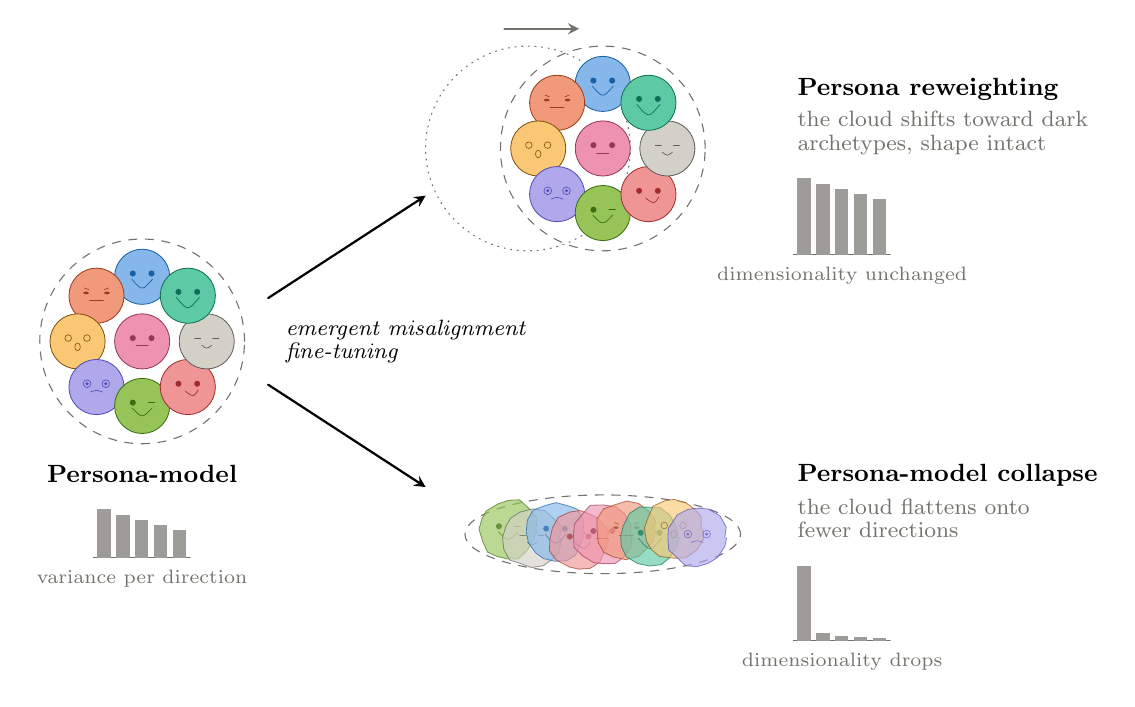
\begin{tikzpicture}[line cap=round, line join=round]

% ════════════════════════════════════════════════════
%  LEFT  —  Persona-model: a round persona cloud, variance spread over many directions
% ════════════════════════════════════════════════════

\draw[labelgray, dashed, thin] (0,0) circle (1.3);
\faceNeutral{0.000}{0.000}{0.35}
\faceHappy{0.000}{0.820}{0.35}
\faceStern{-0.580}{0.580}{0.35}
\faceSurprised{-0.820}{0.000}{0.35}
\faceWise{-0.580}{-0.580}{0.35}
\faceWink{-0.000}{-0.820}{0.35}
\faceSmirk{0.580}{-0.580}{0.35}
\faceSleepy{0.820}{-0.000}{0.35}
\faceGrin{0.580}{0.580}{0.35}
\node[font=\small\bfseries, anchor=north] at (0,-1.45) {Persona-model};
\draw[labelgray, thin] (-0.62,-2.75) -- (0.61,-2.75);
\fill[labelgray!70] (-0.57,-2.75) rectangle (-0.40,-2.13);
\fill[labelgray!70] (-0.33,-2.75) rectangle (-0.16,-2.20);
\fill[labelgray!70] (-0.09,-2.75) rectangle (0.08,-2.27);
\fill[labelgray!70] (0.15,-2.75) rectangle (0.32,-2.33);
\fill[labelgray!70] (0.39,-2.75) rectangle (0.56,-2.39);
\node[font=\scriptsize, text=labelgray, anchor=north] at (-0.00,-2.78) {variance per direction};

% ════════════════════════════════════════════════════
%  FORK
% ════════════════════════════════════════════════════

\draw[-stealth, black, thick] (1.6,0.55) -- (3.6,1.85);
\draw[-stealth, black, thick] (1.6,-0.55) -- (3.6,-1.85);
\node[black, font=\footnotesize\itshape, align=left, anchor=west] at (1.7,0)
  {emergent misalignment\\[-1pt]fine-tuning};

% ════════════════════════════════════════════════════
%  TOP RIGHT  —  Persona reweighting: rigid shift, shape intact
%  dotted circle = where the cloud was; dashed circle = where it is
% ════════════════════════════════════════════════════

\begin{scope}[shift={(4.9,2.45)}]
\draw[labelgray, dotted, thin] (0,0) circle (1.3);
\draw[-stealth, labelgray, thick] (-0.3,1.52) -- (0.65,1.52);
\begin{scope}[shift={(0.95,0)}]
\draw[labelgray, dashed, thin] (0,0) circle (1.3);
\faceNeutral{0.000}{0.000}{0.35}
\faceHappy{0.000}{0.820}{0.35}
\faceStern{-0.580}{0.580}{0.35}
\faceSurprised{-0.820}{0.000}{0.35}
\faceWise{-0.580}{-0.580}{0.35}
\faceWink{-0.000}{-0.820}{0.35}
\faceSmirk{0.580}{-0.580}{0.35}
\faceSleepy{0.820}{-0.000}{0.35}
\faceGrin{0.580}{0.580}{0.35}
\end{scope}
\begin{scope}[shift={(0.95+2.35,0)}]
\node[font=\small\bfseries, anchor=west] at (0,0.75) {Persona reweighting};
\node[font=\footnotesize, text=labelgray, anchor=west, align=left] at (0,0.2)
  {the cloud shifts toward dark\\[-1pt]archetypes, shape intact};
\draw[labelgray, thin] (0.07,-1.35) -- (1.30,-1.35);
\fill[labelgray!70] (0.12,-1.35) rectangle (0.29,-0.38);
\fill[labelgray!70] (0.36,-1.35) rectangle (0.53,-0.45);
\fill[labelgray!70] (0.60,-1.35) rectangle (0.77,-0.52);
\fill[labelgray!70] (0.84,-1.35) rectangle (1.01,-0.58);
\fill[labelgray!70] (1.08,-1.35) rectangle (1.25,-0.64);
\node[font=\scriptsize, text=labelgray, anchor=north] at (0.69,-1.38) {dimensionality unchanged};
\end{scope}
\end{scope}

% ════════════════════════════════════════════════════
%  BOTTOM RIGHT  —  Persona-model collapse: the cloud flattens onto fewer directions
% ════════════════════════════════════════════════════

\pgfmathsetseed{42}
\tikzset{facestyle/.style={%
    decorate,
    decoration={random steps, segment length=4pt, amplitude=0.8pt}}}
\begin{scope}[shift={(5.85,-2.45)}]
\draw[labelgray, dashed, thin] (0,0) ellipse (1.75 and 0.5);
\faceWink[opacity=0.65]{-1.200}{0.060}{0.35}
\faceSleepy[opacity=0.65]{-0.900}{-0.050}{0.35}
\faceHappy[opacity=0.65]{-0.600}{0.030}{0.35}
\faceSmirk[opacity=0.65]{-0.300}{-0.070}{0.35}
\faceNeutral[opacity=0.65]{0.000}{0.000}{0.35}
\faceStern[opacity=0.65]{0.300}{0.050}{0.35}
\faceGrin[opacity=0.65]{0.600}{-0.030}{0.35}
\faceSurprised[opacity=0.65]{0.900}{0.070}{0.35}
\faceWise[opacity=0.65]{1.200}{-0.040}{0.35}
\tikzset{facestyle/.style={}}
\begin{scope}[shift={(2.35,0)}]
\node[font=\small\bfseries, anchor=west] at (0,0.75) {Persona-model collapse};
\node[font=\footnotesize, text=labelgray, anchor=west, align=left] at (0,0.2)
  {the cloud flattens onto\\[-1pt]fewer directions};
\draw[labelgray, thin] (0.07,-1.35) -- (1.30,-1.35);
\fill[labelgray!70] (0.12,-1.35) rectangle (0.29,-0.40);
\fill[labelgray!70] (0.36,-1.35) rectangle (0.53,-1.25);
\fill[labelgray!70] (0.60,-1.35) rectangle (0.77,-1.29);
\fill[labelgray!70] (0.84,-1.35) rectangle (1.01,-1.31);
\fill[labelgray!70] (1.08,-1.35) rectangle (1.25,-1.32);
\node[font=\scriptsize, text=labelgray, anchor=north] at (0.69,-1.3800000000000001) {dimensionality drops};
\end{scope}
\end{scope}

\end{tikzpicture}
\end{document}
